\documentclass{report}
\usepackage{enumitem}
\usepackage{amsmath}
\usepackage{booktabs}
\usepackage{fancyhdr}
\usepackage{tikz}
\usetikzlibrary{arrows.meta}
\usetikzlibrary{calc,positioning,shapes.multipart,shapes}
\usepackage[margin=1in]{geometry}

\renewcommand{\it}[1]{\textit{{#1}}}
\renewcommand{\bf}[1]{\textbf{{#1}}}
\renewcommand{\tt}[1]{\texttt{{#1}}}

\newcommand{\ib}[1]{\it{\bf{{#1}}}}

\pagestyle{fancy}
\fancyhf{}

\fancyhead[L]{\bf{Computer Science 143}}
\fancyhead[C]{\it{Homework 1}}
\fancyhead[R]{\bf{Warren Kim}}
\setlength{\headsep}{0.1in}

\tikzset{
    basic/.style={
        draw,
        rectangle split,
        rectangle split parts=2,
        rectangle split part fill={blue!20,white},
        minimum width=2.5cm,
        text width=2cm,
        align=left,
        font=\itshape
    }
}

\begin{document}
\vspace{2em}

\paragraph{Response:}
No. $T_1$ does not finish completely before $T_2$ starts.
\vspace{2em}

\paragraph{Response:}
We write(A) in $T_1$ before $T_2$ read(A), so $T_1 \to T_2$. But we read(B)
in $T_2$ before $T_1$ write(B), so $T_2 \to T_1$. Therefore,we have

{
    \centering
    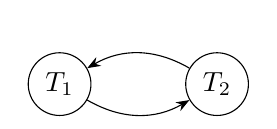
\begin{tikzpicture}[>=Stealth, node distance=2cm]
        \node[circle, draw] (A) {$T_1$};
        \node[circle, draw] (B) [right of=A] {$T_2$};

        \draw[->, bend right] (A) to (B);
        \draw[->, bend right] (B) to (A);
    \end{tikzpicture}
    \par
}

so there is a cycle, and therefore it is not conflict serializable.
\vspace{2em}

\paragraph{Response:}
We write(A) in $T_1$ before write(A) in $T_2$ and read(A) in $T_3$ so $T_1 \to T_2$.
We write(B) in $T_3$ before read(B) in $T_1, T_2$ so $T_3 \to T_1, T_2$.
Then we get

{
    \centering
    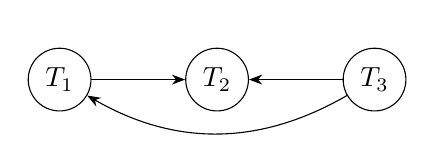
\begin{tikzpicture}[>=Stealth, node distance=2cm]
        \node[circle, draw] (A) {$T_1$};
        \node[circle, draw] (B) [right of=A] {$T_2$};
        \node[circle, draw] (C) [right of=B] {$T_3$};

        \draw[->] (A) to (B);
        \draw[->, bend left] (C) to (A);
        \draw[->] (C) to (B);
    \end{tikzpicture}
    \par
}
\vspace{2em}

\paragraph{Response:}
Yes, there is no cycle in the graph, so we can find a serial ordering of the
transactions. One possible ordering using topological sort is to go from $T_3
\to T_1 \to T_2$. This is because $T_3$ is a source node. $T_1$ becomes a source
node when we visit $T_3$. $T_2$ is the last node left so we visit it last.

\end{document}
